\section{Einsatz von Entwurfsmustern}

"`Entwurfsmuster sind L�sungswissen f�r allgemeine bzw. immer wiederkehrende Probleme [\ldots]. Ein Entwurfsmuster
besteht aus wenigen Klassen, die durch den Einsatz von Delegation und Vererbung eine robuste und modifizierbare L�sung
erm�glichen."'\cite[S. 719]{Bruegge_2004}\\

In Folgenden werden einige Komponenten von Cydonia vorgestellt und erl�utert, wie bei ihrer Entwicklung Entwurfsmuster
zum Einsatz kommen.


\subsection{Equipment-Erzeugung mittels abstrakter Fabrik}
Da die Equipments der Spieler unterschiedlich sein k�nnen und auch in der Zukunft erweiterbar sein sollen, werden sie
von einer Fabrik-Klasse erzeugt. Die Equipments m�ssen in Client und Server jedoch unterschiedliche Implementierungen
haben. Im Client soll das Equipment grafisch dargestellt und Sounds abgespielt werden. Im Server dagegen soll
stattdessen die Auswirkungen der Benutzung berechnet werden. Daher kommt hier das Abstrakte-Fabrik-Muster zum Einsatz.
Das Abstrakte-Fabrik-Muster setzt Spezifikationsvererbung ein, um die Schnittstelle eines Produkts von seiner
Implementierung zu entkoppeln. Um sicherzustellen, dass auf jeder Plattform stets nur die richtigen Objekte erzeugt
werden, also eine konsistente Menge von Objekten vorhanden ist, d�rfen Objekte nur �ber eine Fabrik erzeugt
werden\cite{Bruegge_2004}. Im Fall der Equipments existiert eine ClientEquipmentFactory und eine ServerEquipmentFactory
die jeweils die von AbstractEquipmentFactory geerbten Methoden zur Erzeugung von Pick'n'Place- und Swapper-Equipments
implementieren. Abbildung \ref{figure:equipment_factory} zeigt die Struktur als UML-Klassendiagramm.

\begin{figure}[htbp]
\centering
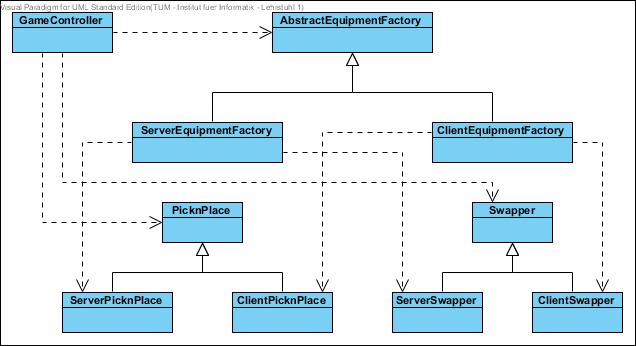
\includegraphics[width=1.0\textwidth]{images/equipment_factory}
\caption[UML-Klassendiagramm: Equipment-Factory]{UML-Klassendiagramm: Equipment-Factory}
\label{figure:equipment_factory}
\end{figure}

\subsection{Szenen-Graph-Erstellung mithilfe des Kompositionsmusters}
\label{subsection:SceneGraph_CompositePattern}
Das Kompositionsmuster ist eine L�sung, um eine solche Hierarchie beliebiger Breite und Tiefe zu repr�sentieren, sodass
sowohl einzelne Objekte als auch Kompositionen von Objekten durch eine gemeinsame Schnittstelle einheitlich behandelt
werden k�nnen. Abbildung \ref{figure:composition_spatial} zeigt die Nutzung des Kompositionsmusters zur Implementierung des
Szenen-Graphen in der jMonkeyEngine3. Die Komponente hei�t hier Spatial. Geometry, die Blatt-Klasse, stellt ein
tats�chliches Objekt in der virtuellen Welt dar, definiert durch Formen und Materialien. Das Kompositum ist Node,
welches wiederum andere Spatials als Kindelemente enthalten kann.\\

\begin{figure}[htbp]
\centering
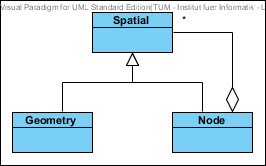
\includegraphics[width=0.6\textwidth]{images/composition_spatial}
\caption[UML-Klassendiagramm: Implementierung Szenen-Graph der jME3]{UML-Klassendiagramm: Implementierung des Szenen-Graph der jME3 unter Verwendung des Kompositionsmusters}
\label{figure:composition_spatial}
\end{figure}

Ein Beispiel f�r die Zusammensetzung der virtuellen Welt aus Spatials, kann anhand des Avatars eines Spieler gegeben
werden. Abbildung \ref{figure:composition_avatar} veranschaulicht die Struktur der Spielfigur. Der Wurzelknoten hat drei
Kindelemente: Kopf, Oberk�rper, Unterk�rper. Der Kopf ist vom Typ Geometry, w�hrend Ober- und Unterk�rper Nodes sind,
die wiederum Kindelemente besitzen, n�mlich Arme, Beine und Torso. Die Unterteilung k�nnte nat�rlich auch noch weiter
gehen: ein Arm k�nnte zum Beispiel wiederum ein Knoten sein, der aus Oberarm, Unterarm und Hand, besteht, wobei die Hand
ebenfalls aus einzelnen Fingern bestehen k�nnte, usw. Beliebig feingliedrige Strukturen sind m�glich, je nach
gew�nschtem Detailgrad der Modelle.

\begin{figure}[htbp]
\centering
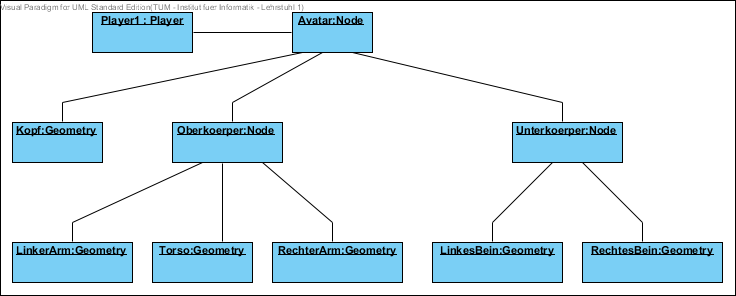
\includegraphics[width=1.0\textwidth]{images/composition_avatar}
\caption[UML-Objektdiagramm: Aufbau des Spieler-Modells]{UML-Objektdiagramm: Aufbau des Spieler-Modells}
\label{figure:composition_avatar}
\end{figure}

\subsection{Event-System mit Beobachtermuster}
Viele Prozesse in Cydonia werden vom Auftreten eines bestimmten Ereignisses angesto�en. Um diese Ereignisse zu verteilen
gibt es eine zentrale Ereignis-Maschine. Objekte, die �ber das Auftreten der Ereignisse informiert werden wollen,
registrieren sich als Beobachter bei der Ereignis-Maschine. Au�erdem stellt sie eine Methode zum Ausl�sen von
Ereignissen in Form von Objekten des Typs Event (oder eines Subtyps) zur Verf�gung. Die Ereignisse werden an jeden
Beobachter in einem eigenen Thread weitergereicht, sodass die Bearbeitung parallel stattfinden kann und eine
aufw�ndigere Bearbeitung nicht die Weiterleitung des Ereignisses an andere Beobachter verz�gert. Abbildung
\ref{figure:event_system} stellt das Ereignis-System als UML-Klassendiagramm dar.

\begin{figure}[htbp]
\centering
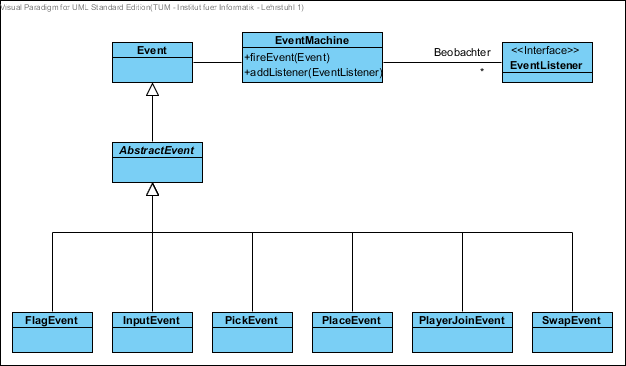
\includegraphics[width=1.0\textwidth]{images/event_system}
\caption[UML-Klassendiagramm: Das Ereignis-System]{UML-Klassendiagramm: Das Ereignis-System}
\label{figure:event_system}
\end{figure}